% Options for packages loaded elsewhere
% Options for packages loaded elsewhere
\PassOptionsToPackage{unicode}{hyperref}
\PassOptionsToPackage{hyphens}{url}
\PassOptionsToPackage{dvipsnames,svgnames,x11names}{xcolor}
%
\documentclass[
  russian,
  letterpaper,
  DIV=11,
  numbers=noendperiod]{scrartcl}
\usepackage{xcolor}
\usepackage{amsmath,amssymb}
\setcounter{secnumdepth}{5}
\usepackage{iftex}
\ifPDFTeX
  \usepackage[T1]{fontenc}
  \usepackage[utf8]{inputenc}
  \usepackage{textcomp} % provide euro and other symbols
\else % if luatex or xetex
  \usepackage{unicode-math} % this also loads fontspec
  \defaultfontfeatures{Scale=MatchLowercase}
  \defaultfontfeatures[\rmfamily]{Ligatures=TeX,Scale=1}
\fi
\usepackage{lmodern}
\ifPDFTeX\else
  % xetex/luatex font selection
\fi
% Use upquote if available, for straight quotes in verbatim environments
\IfFileExists{upquote.sty}{\usepackage{upquote}}{}
\IfFileExists{microtype.sty}{% use microtype if available
  \usepackage[]{microtype}
  \UseMicrotypeSet[protrusion]{basicmath} % disable protrusion for tt fonts
}{}
\makeatletter
\@ifundefined{KOMAClassName}{% if non-KOMA class
  \IfFileExists{parskip.sty}{%
    \usepackage{parskip}
  }{% else
    \setlength{\parindent}{0pt}
    \setlength{\parskip}{6pt plus 2pt minus 1pt}}
}{% if KOMA class
  \KOMAoptions{parskip=half}}
\makeatother
% Make \paragraph and \subparagraph free-standing
\makeatletter
\ifx\paragraph\undefined\else
  \let\oldparagraph\paragraph
  \renewcommand{\paragraph}{
    \@ifstar
      \xxxParagraphStar
      \xxxParagraphNoStar
  }
  \newcommand{\xxxParagraphStar}[1]{\oldparagraph*{#1}\mbox{}}
  \newcommand{\xxxParagraphNoStar}[1]{\oldparagraph{#1}\mbox{}}
\fi
\ifx\subparagraph\undefined\else
  \let\oldsubparagraph\subparagraph
  \renewcommand{\subparagraph}{
    \@ifstar
      \xxxSubParagraphStar
      \xxxSubParagraphNoStar
  }
  \newcommand{\xxxSubParagraphStar}[1]{\oldsubparagraph*{#1}\mbox{}}
  \newcommand{\xxxSubParagraphNoStar}[1]{\oldsubparagraph{#1}\mbox{}}
\fi
\makeatother

\usepackage{color}
\usepackage{fancyvrb}
\newcommand{\VerbBar}{|}
\newcommand{\VERB}{\Verb[commandchars=\\\{\}]}
\DefineVerbatimEnvironment{Highlighting}{Verbatim}{commandchars=\\\{\}}
% Add ',fontsize=\small' for more characters per line
\usepackage{framed}
\definecolor{shadecolor}{RGB}{241,243,245}
\newenvironment{Shaded}{\begin{snugshade}}{\end{snugshade}}
\newcommand{\AlertTok}[1]{\textcolor[rgb]{0.68,0.00,0.00}{#1}}
\newcommand{\AnnotationTok}[1]{\textcolor[rgb]{0.37,0.37,0.37}{#1}}
\newcommand{\AttributeTok}[1]{\textcolor[rgb]{0.40,0.45,0.13}{#1}}
\newcommand{\BaseNTok}[1]{\textcolor[rgb]{0.68,0.00,0.00}{#1}}
\newcommand{\BuiltInTok}[1]{\textcolor[rgb]{0.00,0.23,0.31}{#1}}
\newcommand{\CharTok}[1]{\textcolor[rgb]{0.13,0.47,0.30}{#1}}
\newcommand{\CommentTok}[1]{\textcolor[rgb]{0.37,0.37,0.37}{#1}}
\newcommand{\CommentVarTok}[1]{\textcolor[rgb]{0.37,0.37,0.37}{\textit{#1}}}
\newcommand{\ConstantTok}[1]{\textcolor[rgb]{0.56,0.35,0.01}{#1}}
\newcommand{\ControlFlowTok}[1]{\textcolor[rgb]{0.00,0.23,0.31}{\textbf{#1}}}
\newcommand{\DataTypeTok}[1]{\textcolor[rgb]{0.68,0.00,0.00}{#1}}
\newcommand{\DecValTok}[1]{\textcolor[rgb]{0.68,0.00,0.00}{#1}}
\newcommand{\DocumentationTok}[1]{\textcolor[rgb]{0.37,0.37,0.37}{\textit{#1}}}
\newcommand{\ErrorTok}[1]{\textcolor[rgb]{0.68,0.00,0.00}{#1}}
\newcommand{\ExtensionTok}[1]{\textcolor[rgb]{0.00,0.23,0.31}{#1}}
\newcommand{\FloatTok}[1]{\textcolor[rgb]{0.68,0.00,0.00}{#1}}
\newcommand{\FunctionTok}[1]{\textcolor[rgb]{0.28,0.35,0.67}{#1}}
\newcommand{\ImportTok}[1]{\textcolor[rgb]{0.00,0.46,0.62}{#1}}
\newcommand{\InformationTok}[1]{\textcolor[rgb]{0.37,0.37,0.37}{#1}}
\newcommand{\KeywordTok}[1]{\textcolor[rgb]{0.00,0.23,0.31}{\textbf{#1}}}
\newcommand{\NormalTok}[1]{\textcolor[rgb]{0.00,0.23,0.31}{#1}}
\newcommand{\OperatorTok}[1]{\textcolor[rgb]{0.37,0.37,0.37}{#1}}
\newcommand{\OtherTok}[1]{\textcolor[rgb]{0.00,0.23,0.31}{#1}}
\newcommand{\PreprocessorTok}[1]{\textcolor[rgb]{0.68,0.00,0.00}{#1}}
\newcommand{\RegionMarkerTok}[1]{\textcolor[rgb]{0.00,0.23,0.31}{#1}}
\newcommand{\SpecialCharTok}[1]{\textcolor[rgb]{0.37,0.37,0.37}{#1}}
\newcommand{\SpecialStringTok}[1]{\textcolor[rgb]{0.13,0.47,0.30}{#1}}
\newcommand{\StringTok}[1]{\textcolor[rgb]{0.13,0.47,0.30}{#1}}
\newcommand{\VariableTok}[1]{\textcolor[rgb]{0.07,0.07,0.07}{#1}}
\newcommand{\VerbatimStringTok}[1]{\textcolor[rgb]{0.13,0.47,0.30}{#1}}
\newcommand{\WarningTok}[1]{\textcolor[rgb]{0.37,0.37,0.37}{\textit{#1}}}

\usepackage{longtable,booktabs,array}
\usepackage{calc} % for calculating minipage widths
% Correct order of tables after \paragraph or \subparagraph
\usepackage{etoolbox}
\makeatletter
\patchcmd\longtable{\par}{\if@noskipsec\mbox{}\fi\par}{}{}
\makeatother
% Allow footnotes in longtable head/foot
\IfFileExists{footnotehyper.sty}{\usepackage{footnotehyper}}{\usepackage{footnote}}
\makesavenoteenv{longtable}
\usepackage{graphicx}
\makeatletter
\newsavebox\pandoc@box
\newcommand*\pandocbounded[1]{% scales image to fit in text height/width
  \sbox\pandoc@box{#1}%
  \Gscale@div\@tempa{\textheight}{\dimexpr\ht\pandoc@box+\dp\pandoc@box\relax}%
  \Gscale@div\@tempb{\linewidth}{\wd\pandoc@box}%
  \ifdim\@tempb\p@<\@tempa\p@\let\@tempa\@tempb\fi% select the smaller of both
  \ifdim\@tempa\p@<\p@\scalebox{\@tempa}{\usebox\pandoc@box}%
  \else\usebox{\pandoc@box}%
  \fi%
}
% Set default figure placement to htbp
\def\fps@figure{htbp}
\makeatother



\ifLuaTeX
\usepackage[bidi=basic,provide=*]{babel}
\else
\usepackage[bidi=default,provide=*]{babel}
\fi
% get rid of language-specific shorthands (see #6817):
\let\LanguageShortHands\languageshorthands
\def\languageshorthands#1{}


\setlength{\emergencystretch}{3em} % prevent overfull lines

\providecommand{\tightlist}{%
  \setlength{\itemsep}{0pt}\setlength{\parskip}{0pt}}



 


\usepackage{fontspec}

\setsansfont{Palatino Linotype}[
    Path=../files/palatino/,
    Extension = .ttf,
    UprightFont=palatino-Roman,
    BoldFont=palatino-Bold,
    ItalicFont=palatino-Italic,
    BoldItalicFont=palatino-BoldItalic
]
\setmainfont{Palatino Linotype}[
    Path=../files/palatino/,
    Extension = .ttf,
    UprightFont=palatino-Roman,
    BoldFont=palatino-Bold,
    ItalicFont=palatino-Italic,
    BoldItalicFont=palatino-BoldItalic
]

\usepackage[textwidth=0.86\paperwidth, textheight=0.86\paperheight]{geometry}
\usepackage{fancyhdr}
\usepackage{hyperref}
\usepackage{fontawesome5}
\usepackage{graphicx}
\usepackage{amssymb}
\usepackage{amsmath}
\graphicspath{{../files/}}

\newcommand{\R}{\mathbb{R}}

% \pagenumbering{gobble}
\pagestyle{fancy}
\fancyhead{} % clear all header fields
\fancyhead[R]{\href{https://cu25.fmin.xyz}{\faGem[regular]} \hspace{0.04cm} \href{https://github.com/MerkulovDaniil/cu25}{\faGithub} \hspace{0.07cm} \href{https://t.me/fminxyz}{\faTelegram}}
\fancyhead[L]{\href{https://fmin.xyz}{
\includegraphics[height=0.35cm]{logo.pdf}} ~ 
\includegraphics[height=0.35cm]{logo_cu.pdf} \hspace{2pt} \textbf{Оптимизация для всех! ЦУ. 2025}}
\KOMAoption{captions}{tableheading}
\makeatletter
\@ifpackageloaded{tcolorbox}{}{\usepackage[skins,breakable]{tcolorbox}}
\@ifpackageloaded{fontawesome5}{}{\usepackage{fontawesome5}}
\definecolor{quarto-callout-color}{HTML}{909090}
\definecolor{quarto-callout-note-color}{HTML}{0758E5}
\definecolor{quarto-callout-important-color}{HTML}{CC1914}
\definecolor{quarto-callout-warning-color}{HTML}{EB9113}
\definecolor{quarto-callout-tip-color}{HTML}{00A047}
\definecolor{quarto-callout-caution-color}{HTML}{FC5300}
\definecolor{quarto-callout-color-frame}{HTML}{acacac}
\definecolor{quarto-callout-note-color-frame}{HTML}{4582ec}
\definecolor{quarto-callout-important-color-frame}{HTML}{d9534f}
\definecolor{quarto-callout-warning-color-frame}{HTML}{f0ad4e}
\definecolor{quarto-callout-tip-color-frame}{HTML}{02b875}
\definecolor{quarto-callout-caution-color-frame}{HTML}{fd7e14}
\makeatother
\makeatletter
\@ifpackageloaded{caption}{}{\usepackage{caption}}
\AtBeginDocument{%
\ifdefined\contentsname
  \renewcommand*\contentsname{Содержание}
\else
  \newcommand\contentsname{Содержание}
\fi
\ifdefined\listfigurename
  \renewcommand*\listfigurename{Список Иллюстраций}
\else
  \newcommand\listfigurename{Список Иллюстраций}
\fi
\ifdefined\listtablename
  \renewcommand*\listtablename{Список Таблиц}
\else
  \newcommand\listtablename{Список Таблиц}
\fi
\ifdefined\figurename
  \renewcommand*\figurename{Рисунок}
\else
  \newcommand\figurename{Рисунок}
\fi
\ifdefined\tablename
  \renewcommand*\tablename{Таблица}
\else
  \newcommand\tablename{Таблица}
\fi
}
\@ifpackageloaded{float}{}{\usepackage{float}}
\floatstyle{ruled}
\@ifundefined{c@chapter}{\newfloat{codelisting}{h}{lop}}{\newfloat{codelisting}{h}{lop}[chapter]}
\floatname{codelisting}{Список}
\newcommand*\listoflistings{\listof{codelisting}{Список Каталогов}}
\makeatother
\makeatletter
\makeatother
\makeatletter
\@ifpackageloaded{caption}{}{\usepackage{caption}}
\@ifpackageloaded{subcaption}{}{\usepackage{subcaption}}
\makeatother
\usepackage{bookmark}
\IfFileExists{xurl.sty}{\usepackage{xurl}}{} % add URL line breaks if available
\urlstyle{same}
\hypersetup{
  pdftitle={Вспоминаем линейную алгебру. Скорости сходимости.},
  pdfauthor={Даня Меркулов},
  pdflang={ru},
  colorlinks=true,
  linkcolor={blue},
  filecolor={Maroon},
  citecolor={Blue},
  urlcolor={Blue},
  pdfcreator={LaTeX via pandoc}}


\title{Вспоминаем линейную алгебру. Скорости сходимости.}
\author{Даня Меркулов}
\date{}
\begin{document}
\maketitle


\section{Вспоминаем линейную
алгебру}\label{ux432ux441ux43fux43eux43cux438ux43dux430ux435ux43c-ux43bux438ux43dux435ux439ux43dux443ux44e-ux430ux43bux433ux435ux431ux440ux443}

\subsection{Векторы и
матрицы}\label{ux432ux435ux43aux442ux43eux440ux44b-ux438-ux43cux430ux442ux440ux438ux446ux44b}

Мы будем считать, что все векторы являются столбцами по умолчанию.
Пространство векторов длины \(n\) обозначается \(\mathbb{R}^n\), а
пространство матриц размера \(m \times n\) с вещественными элементами
обозначается \(\mathbb{R}^{m \times n}\). То есть \footnote{Подробный
  вводный курс по прикладной линейной алгебре можно найти в книге
  \href{https://web.stanford.edu/~boyd/vmls/}{Introduction to Applied
  Linear Algebra -- Vectors, Matrices, and Least Squares} - книга от
  Stephen Boyd \& Lieven Vandenberghe, которая указана в источнике.
  Также полезен материал по линейной алгебре приведенный в приложении А
  книги Numerical Optimization by Jorge Nocedal Stephen J. Wright.}:

\begin{equation}\phantomsection\label{eq-vector}{
x = \begin{bmatrix}
x_1 \\
x_2 \\
\vdots \\
x_n
\end{bmatrix} \quad x^T = \begin{bmatrix}
x_1 & x_2 & \dots & x_n
\end{bmatrix} \quad x \in \mathbb{R}^n, x_i \in \mathbb{R}
}\end{equation}

Аналогично, если \(A \in \mathbb{R}^{m \times n}\) мы обозначаем
транспонирование как \(A^T \in \mathbb{R}^{n \times m}\): \[
A = \begin{bmatrix}
a_{11} & a_{12} & \dots & a_{1n} \\
a_{21} & a_{22} & \dots & a_{2n} \\
\vdots & \vdots & \ddots & \vdots \\
a_{m1} & a_{m2} & \dots & a_{mn}
\end{bmatrix} \quad A^T = \begin{bmatrix}
a_{11} & a_{21} & \dots & a_{m1} \\
a_{12} & a_{22} & \dots & a_{m2} \\
\vdots & \vdots & \ddots & \vdots \\
a_{1n} & a_{2n} & \dots & a_{mn}
\end{bmatrix} \quad A \in \mathbb{R}^{m \times n}, a_{ij} \in \mathbb{R}
\] Мы будем писать \(x \geq 0\) и \(x \neq 0\) для обозначения
покомпонентных неравенств

\begin{figure}

\centering{

\pandocbounded{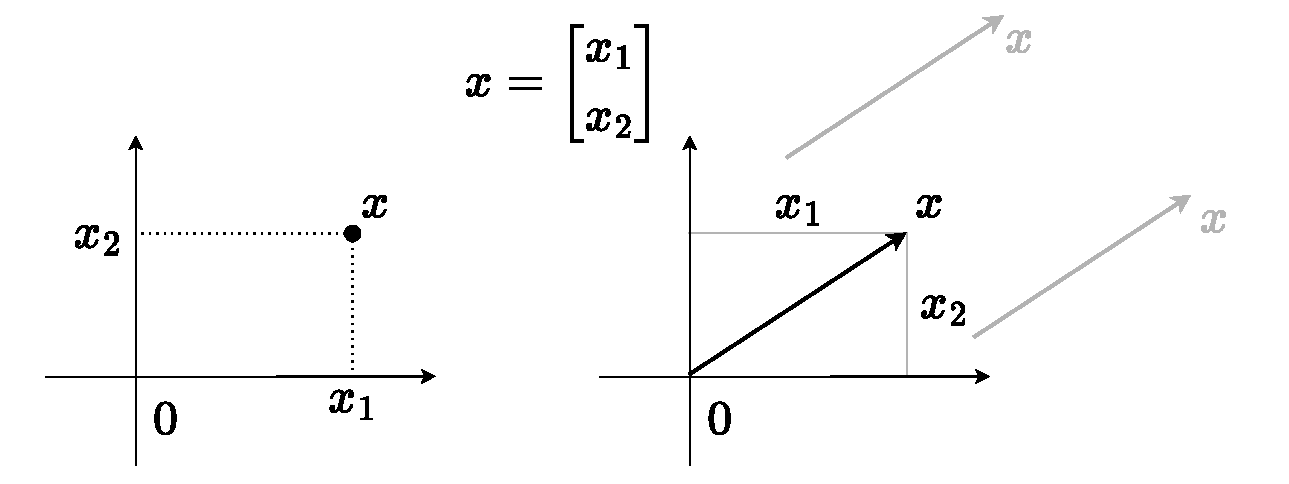
\includegraphics[keepaspectratio]{vector.pdf}}

}

\caption{\label{fig-vector}Эквивалентные представления вектора}

\end{figure}%

Матрица \(A\) называется симметричной, если \(A = A^T\). Обозначается
как \(A \in \mathbb{S}^n\) (множество квадратных симметричных матриц
размерности \(n\)). Заметим, что только квадратная матрица может быть
симметричной по определению.

Матрица \(A \in \mathbb{S}^n\) называется \textbf{положительно
(отрицательно) определенной}, если для всех
\(x \neq 0 : x^T Ax > (<) 0\). Обозначается как \(A \succ (\prec) 0\).
Множество таких матриц обозначается как
\(\mathbb{S}^n_{++} (\mathbb{S}^n_{- -})\)

Матрица \(A \in \mathbb{S}^n\) называется \textbf{положительно
(отрицательно) полуопределенной}, если для всех
\(x : x^T Ax \geq (\leq) 0\). Обозначается как
\(A \succeq (\preceq) 0\). Множество таких матриц обозначается как
\(\mathbb{S}^n_{+} (\mathbb{S}^n_{-})\)

\begin{tcolorbox}[enhanced jigsaw, breakable, toptitle=1mm, title=\textcolor{quarto-callout-color}{\faInfo}\hspace{0.5em}{Question}, colbacktitle=quarto-callout-color!10!white, opacityback=0, colback=white, left=2mm, coltitle=black, rightrule=.15mm, opacitybacktitle=0.6, colframe=quarto-callout-color-frame, bottomtitle=1mm, titlerule=0mm, arc=.35mm, bottomrule=.15mm, toprule=.15mm, leftrule=.75mm]

Верно ли, что положительно определенная матрица имеет все положительные
элементы?

\end{tcolorbox}

\begin{tcolorbox}[enhanced jigsaw, breakable, toptitle=1mm, title=\textcolor{quarto-callout-color}{\faInfo}\hspace{0.5em}{Question}, colbacktitle=quarto-callout-color!10!white, opacityback=0, colback=white, left=2mm, coltitle=black, rightrule=.15mm, opacitybacktitle=0.6, colframe=quarto-callout-color-frame, bottomtitle=1mm, titlerule=0mm, arc=.35mm, bottomrule=.15mm, toprule=.15mm, leftrule=.75mm]

Верно ли, что если матрица симметрична, то она должна быть положительно
определенной?

\end{tcolorbox}

\begin{tcolorbox}[enhanced jigsaw, breakable, toptitle=1mm, title=\textcolor{quarto-callout-color}{\faInfo}\hspace{0.5em}{Question}, colbacktitle=quarto-callout-color!10!white, opacityback=0, colback=white, left=2mm, coltitle=black, rightrule=.15mm, opacitybacktitle=0.6, colframe=quarto-callout-color-frame, bottomtitle=1mm, titlerule=0mm, arc=.35mm, bottomrule=.15mm, toprule=.15mm, leftrule=.75mm]

Верно ли, что если матрица положительно определена, то она должна быть
симметричной?

\end{tcolorbox}

\subsection{Матричное умножение
(matmul)}\label{ux43cux430ux442ux440ux438ux447ux43dux43eux435-ux443ux43cux43dux43eux436ux435ux43dux438ux435-matmul}

Пусть \(A\) - матрица размера \(m \times n\), а \(B\) - матрица размера
\(n \times p\), тогда их произведение \(AB\) равно: \[
C = AB
\] Тогда \(C\) - матрица размера \(m \times p\), элемент \((i, j)\)
которой равен: \[
c_{ij} = \sum_{k=1}^n a_{ik}b_{kj}.
\]

Эта операция в наивной форме требует \(\mathcal{O}(n^3)\) арифметических
операций, где \(n\) обычно считается наибольшей размерностью матриц.

\begin{tcolorbox}[enhanced jigsaw, breakable, toptitle=1mm, title=\textcolor{quarto-callout-color}{\faInfo}\hspace{0.5em}{Question}, colbacktitle=quarto-callout-color!10!white, opacityback=0, colback=white, left=2mm, coltitle=black, rightrule=.15mm, opacitybacktitle=0.6, colframe=quarto-callout-color-frame, bottomtitle=1mm, titlerule=0mm, arc=.35mm, bottomrule=.15mm, toprule=.15mm, leftrule=.75mm]

Возможно ли умножить две матрицы быстрее, чем за \(\mathcal{O}(n^3)\)?
Как насчет \(\mathcal{O}(n^2)\), \(\mathcal{O}(n)\)?

\end{tcolorbox}

\subsection{Умножение матрицы на вектор
(matvec)}\label{ux443ux43cux43dux43eux436ux435ux43dux438ux435-ux43cux430ux442ux440ux438ux446ux44b-ux43dux430-ux432ux435ux43aux442ux43eux440-matvec}

Пусть \(A\) - матрица размера \(m \times n\), а \(x\) - вектор длины
\(n\), тогда \(i\)-й элемент произведения \(Ax\) равен: \[
z = Ax
\] равен: \[
z_i = \sum_{k=1}^n a_{ik}x_k
\]

Эта операция в наивной форме требует \(\mathcal{O}(n^2)\) арифметических
операций, где \(n\) обычно считается наибольшей размерностью входов.

Отметим, что:

\begin{itemize}
\tightlist
\item
  \(C = AB \quad C^T = B^T A^T\)
\item
  \(AB \neq BA\)
\item
  \(e^{A} =\sum\limits_{k=0}^{\infty }{1 \over k!}A^{k}\)
\item
  \(e^{A+B} \neq e^{A} e^{B}\) (но если \(A\) и \(B\) коммутируют, то
  есть \(AB = BA\), то \(e^{A+B} = e^{A} e^{B}\))
\item
  \(\langle x, Ay\rangle = \langle A^T x, y\rangle\)
\end{itemize}

\subsection{Нормы}\label{ux43dux43eux440ux43cux44b}

Норма - это \textbf{количественная мера малости вектора} и обычно
обозначается как \(\Vert x \Vert\).

Норма должна удовлетворять определенным свойствам:

\begin{enumerate}
\def\labelenumi{\arabic{enumi}.}
\tightlist
\item
  \(\Vert \alpha x \Vert = \vert \alpha\vert \Vert x \Vert\),
  \(\alpha \in \mathbb{R}\)
\item
  \(\Vert x + y \Vert \leq \Vert x \Vert + \Vert y \Vert\) (неравенство
  треугольника)
\item
  Если \(\Vert x \Vert = 0\), то \(x = 0\)
\end{enumerate}

Расстояние между двумя векторами определяется как \[ 
d(x, y) = \Vert x - y \Vert. 
\] Наиболее широко используемой нормой является \textbf{Евклидова
норма}: \[
\Vert x \Vert_2 = \sqrt{\sum_{i=1}^n |x_i|^2},
\] которая соответствует расстоянию в нашей реальной жизни. Если векторы
имеют комплексные элементы, мы используем их модуль. Евклидова норма,
или \(2\)-норма, является подклассом важного класса \(p\)-норм:

\[
\Vert x \Vert_p = \Big(\sum_{i=1}^n |x_i|^p\Big)^{1/p}. 
\]

\begin{center}\rule{0.5\linewidth}{0.5pt}\end{center}

\subsection{\texorpdfstring{\(p\)-норма
вектора}{p-норма вектора}}\label{p-ux43dux43eux440ux43cux430-ux432ux435ux43aux442ux43eux440ux430}

Существуют два очень важных частных случая. Бесконечность-норма, или
норма Чебышева, определяется как максимальное абсолютное значение
элемента вектора: \[
\Vert x \Vert_{\infty} = \max_i | x_i| 
\]

\(l_1\) норма (или \textbf{манхэттенское расстояние}) определяется как
сумма модулей элементов вектора \(x\):

\[
\Vert x \Vert_1 = \sum_i |x_i| 
\]

\(l_1\) норма играет очень важную роль: она все связана с методами
\textbf{compressed sensing}, которые появились в середине 00-х как одна
из популярных тем исследований. Код для изображения ниже доступен
\href{https://colab.research.google.com/github/MerkulovDaniil/optim/blob/master/assets/Notebooks/Balls_p_norm.ipynb}{\emph{здесь:}}.
Также посмотрите
\href{https://fmin.xyz/docs/theory/balls_norm.mp4}{\emph{это}} видео.

\begin{figure}[H]

{\centering \pandocbounded{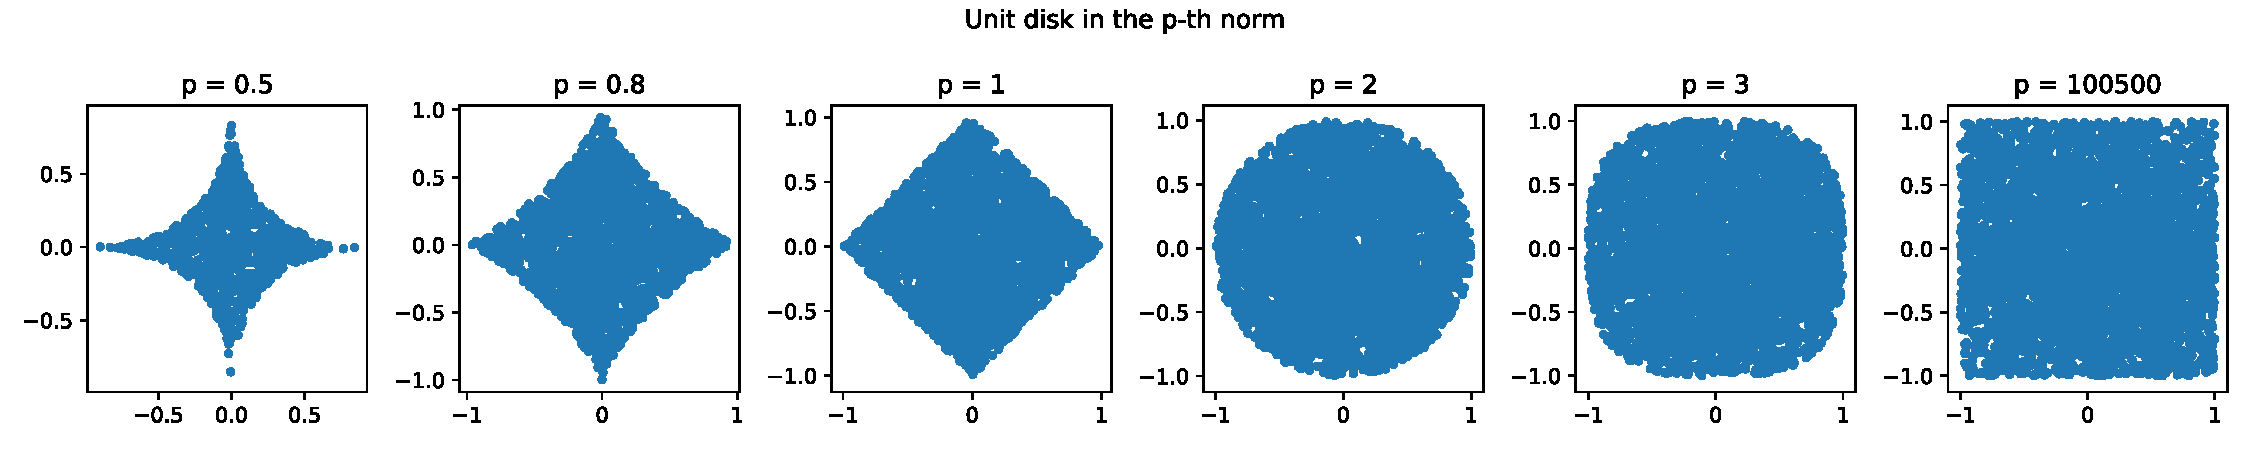
\includegraphics[keepaspectratio]{p_balls.pdf}}

}

\caption{Шары в разных нормах на плоскости}

\end{figure}%

\subsection{Матричные
нормы}\label{ux43cux430ux442ux440ux438ux447ux43dux44bux435-ux43dux43eux440ux43cux44b}

В некотором смысле между матрицами и векторами нет большой разницы (вы
можете векторизовать матрицу), и здесь появляется самая простая
матричная норма \textbf{Фробениуса}: \[
\Vert A \Vert_F = \left(\sum_{i=1}^m \sum_{j=1}^n |a_{ij}|^2\right)^{1/2}
\]

Спектральная норма, \(\Vert A \Vert_2\) является одной из наиболее
широко используемых матричных норм (наряду с нормой Фробениуса).

\[
\Vert A \Vert_2 = \sup_{x \ne 0} \frac{\Vert A x \Vert_2}{\Vert x \Vert_{2}},
\]

Она не может быть вычислена непосредственно из элементов с помощью
простой формулы, как в случае нормы Фробениуса, однако, существуют
эффективные алгоритмы для ее вычисления. Она напрямую связана с
\textbf{сингулярным разложением} (SVD) матрицы. Для неё справедливо:

\[
\Vert A \Vert_2 = \sigma_1(A) = \sqrt{\lambda_{\max}(A^TA)}
\]

где \(\sigma_1(A)\) - наибольшее сингулярное значение матрицы \(A\).

\subsection{Скалярное
произведение}\label{ux441ux43aux430ux43bux44fux440ux43dux43eux435-ux43fux440ux43eux438ux437ux432ux435ux434ux435ux43dux438ux435}

Стандартное \textbf{скалярное произведение} между векторами \(x\) и
\(y\) из \(\mathbb{R}^n\) равно: \[
\langle x, y \rangle = x^T y = \sum\limits_{i=1}^n x_i y_i = y^T x =  \langle y, x \rangle
\]

Здесь \(x_i\) и \(y_i\) - \(i\)-ые компоненты соответствующих векторов.

\begin{tcolorbox}[enhanced jigsaw, breakable, toptitle=1mm, title=\textcolor{quarto-callout-color}{\faInfo}\hspace{0.5em}{Example}, colbacktitle=quarto-callout-color!10!white, opacityback=0, colback=white, left=2mm, coltitle=black, rightrule=.15mm, opacitybacktitle=0.6, colframe=quarto-callout-color-frame, bottomtitle=1mm, titlerule=0mm, arc=.35mm, bottomrule=.15mm, toprule=.15mm, leftrule=.75mm]

Докажите, что вы можете переставить матрицу внутри скалярного
произведения с транспонированием:
\(\langle x, Ay\rangle = \langle A^Tx, y\rangle\) и
\(\langle x, yB\rangle = \langle xB^T, y\rangle\)

\end{tcolorbox}

\subsection{Скалярное произведение
матриц}\label{ux441ux43aux430ux43bux44fux440ux43dux43eux435-ux43fux440ux43eux438ux437ux432ux435ux434ux435ux43dux438ux435-ux43cux430ux442ux440ux438ux446}

Стандартное \textbf{скалярное произведение} между матрицами \(X\) и
\(Y\) из \(\mathbb{R}^{m \times n}\) равно:

\[
\langle X, Y \rangle = \text{tr}(X^T Y) = \sum\limits_{i=1}^m\sum\limits_{j=1}^n X_{ij} Y_{ij} =  \text{tr}(Y^T X) =  \langle Y, X \rangle
\]

\begin{tcolorbox}[enhanced jigsaw, breakable, toptitle=1mm, title=\textcolor{quarto-callout-color}{\faInfo}\hspace{0.5em}{Question}, colbacktitle=quarto-callout-color!10!white, opacityback=0, colback=white, left=2mm, coltitle=black, rightrule=.15mm, opacitybacktitle=0.6, colframe=quarto-callout-color-frame, bottomtitle=1mm, titlerule=0mm, arc=.35mm, bottomrule=.15mm, toprule=.15mm, leftrule=.75mm]

Существует ли связь между нормой Фробениуса \(\Vert \cdot \Vert_F\) и
скалярным произведением между матрицами
\(\langle \cdot, \cdot \rangle\)?

\end{tcolorbox}

\subsection{Собственные вектора и собственные
значения}\label{ux441ux43eux431ux441ux442ux432ux435ux43dux43dux44bux435-ux432ux435ux43aux442ux43eux440ux430-ux438-ux441ux43eux431ux441ux442ux432ux435ux43dux43dux44bux435-ux437ux43dux430ux447ux435ux43dux438ux44f}

Число \(\lambda\) является собственным значением квадратной матрицы
\(A\) размера \(n \times n\), если существует ненулевой вектор \(q\)
такой, что \[ 
Aq = \lambda q. 
\]

Вектор \(q\) называется собственным вектором матрицы \(A\). Матрица
\(A\) невырожденная, если ни одно из её собственных значений не равно
нулю. Собственные значения симметричных матриц являются вещественными
числами, в то время как несимметричные матрицы могут иметь комплексные
собственные значения. Если матрица положительно определена и
симметрична, то все её собственные значения являются положительными
вещественными числами.

\subsection{Собственные вектора и собственные
значения}\label{ux441ux43eux431ux441ux442ux432ux435ux43dux43dux44bux435-ux432ux435ux43aux442ux43eux440ux430-ux438-ux441ux43eux431ux441ux442ux432ux435ux43dux43dux44bux435-ux437ux43dux430ux447ux435ux43dux438ux44f-1}

\begin{tcolorbox}[enhanced jigsaw, breakable, toptitle=1mm, title=\textcolor{quarto-callout-color}{\faInfo}\hspace{0.5em}{Theorem}, colbacktitle=quarto-callout-color!10!white, opacityback=0, colback=white, left=2mm, coltitle=black, rightrule=.15mm, opacitybacktitle=0.6, colframe=quarto-callout-color-frame, bottomtitle=1mm, titlerule=0mm, arc=.35mm, bottomrule=.15mm, toprule=.15mm, leftrule=.75mm]

\[
A \succeq (\succ) 0 \Leftrightarrow \text{все собственные значения } A \text{ } \geq (>) 0 
\]

\begin{quote}
\textbf{Proof}

\begin{enumerate}
\def\labelenumi{\arabic{enumi}.}
\tightlist
\item
  \(\rightarrow\) Предположим, что некоторое собственное значение
  \(\lambda\) отрицательно, и пусть \(x\) обозначает соответствующий
  собственный вектор. Тогда \[
  Ax = \lambda x \rightarrow x^T Ax = \lambda x^T x < 0
  \] что противоречит условию \(A \succeq 0\).
\item
  \(\leftarrow\) Для любой симметричной матрицы мы можем выбрать набор
  собственных векторов \(v_1, \dots, v_n\), которые образуют
  ортонормированный базис в \(\mathbb{R}^n\). Возьмем любой вектор
  \(x \in \mathbb{R}^n\). \[
  \begin{split}
  x^T A x &= (\alpha_1 v_1 + \ldots + \alpha_n v_n)^T A (\alpha_1 v_1 + \ldots + \alpha_n v_n)\\
  &= \sum \alpha_i^2 v_i^T A v_i = \sum \alpha_i^2 \lambda_i v_i^T v_i \geq 0
  \end{split}
  \] Здесь мы использовали тот факт, что \(v_i^T v_j = 0\), для
  \(i \neq j\).
\end{enumerate}
\end{quote}

\end{tcolorbox}

\subsection{Спектральное разложение
(eigendecomposition)}\label{ux441ux43fux435ux43aux442ux440ux430ux43bux44cux43dux43eux435-ux440ux430ux437ux43bux43eux436ux435ux43dux438ux435-eigendecomposition}

Пусть \(A \in S_n\), т.е. \(A\) - вещественная симметричная матрица
размера \(n \times n\). Тогда \(A\) может быть разложена как

\[ 
A = Q\Lambda Q^T,
\]

где \(Q \in \mathbb{R}^{n \times n}\) ортогональная, т.е. удовлетворяет
\(Q^T Q = I\), и
\(\Lambda = \text{diag}(\lambda_1, \ldots , \lambda_n)\). Вещественные
числа \(\lambda_i\) являются собственными значениями \(A\) и являются
корнями характеристического полинома \(\text{det}(A - \lambda I)\).
Столбцы \(Q\) образуют ортонормированный набор собственных векторов
\(A\). Такое разложение называется спектральным. \footnote{Хорошая
  шпаргалка с разложением матриц доступна на сайте курса по линейной
  алгебре
  \href{https://nla.skoltech.ru/_files/decompositions.pdf}{website}.}

Мы обычно упорядочиваем вещественные собственные значения как
\(\lambda_1 \geq \lambda_2 \geq \ldots \geq \lambda_n\). Мы используем
обозначение \(\lambda_i(A)\) для обозначения \(i\)-го наибольшего
собственного значения \(A \in S\). Мы обычно пишем наибольшее или
максимальное собственное значение как
\(\lambda_1(A) = \lambda_{\text{max}}(A)\), и наименьшее или минимальное
собственное значение как \(\lambda_n(A) = \lambda_{\text{min}}(A)\).

\subsection{Собственные
значения}\label{ux441ux43eux431ux441ux442ux432ux435ux43dux43dux44bux435-ux437ux43dux430ux447ux435ux43dux438ux44f}

Наибольшее и наименьшее вещественныесобственные значения удовлетворяют

\[
\lambda_{\text{min}} (A) = \inf_{x \neq 0} \dfrac{x^T Ax}{x^T x}, \qquad \lambda_{\text{max}} (A) = \sup_{x \neq 0} \dfrac{x^T Ax}{x^T x}
\]

и, следовательно, \(\forall x \in \mathbb{R}^n\) (соотношение Рэлея):

\[
\lambda_{\text{min}} (A) x^T x \leq x^T Ax \leq \lambda_{\text{max}} (A) x^T x
\]

\textbf{Число обусловленности} невырожденной матрицы определяется как

\[
\kappa(A) = \|A\|\|A^{-1}\|
\]

Если мы используем спектральную матричную норму, мы можем получить:

\[
\kappa(A) = \dfrac{\sigma_{\text{max}}(A)}{\sigma _{\text{min}}(A)}
\]

Если, кроме того, \(A \in \mathbb{S}^n_{++}\):
\(\kappa(A) = \dfrac{\lambda_{\text{max}}(A)}{\lambda_{\text{min}}(A)}\)

\subsection{Число
обусловленности}\label{ux447ux438ux441ux43bux43e-ux43eux431ux443ux441ux43bux43eux432ux43bux435ux43dux43dux43eux441ux442ux438}

\pandocbounded{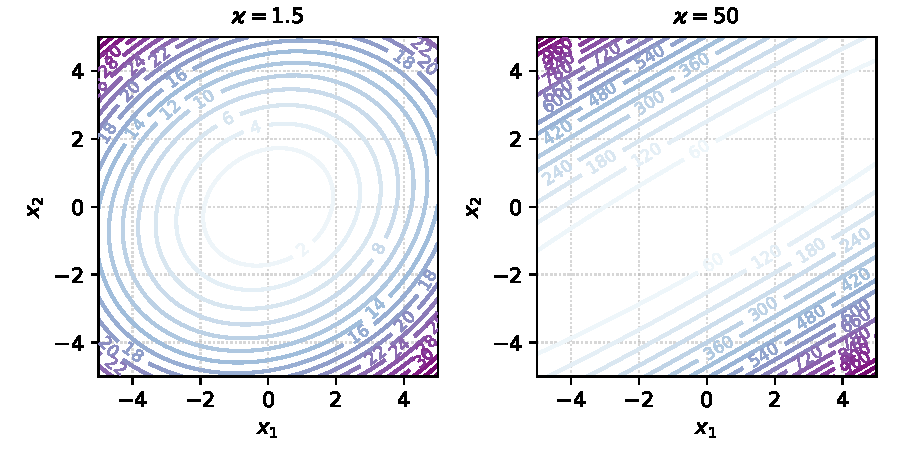
\includegraphics[keepaspectratio]{conditions.pdf}}

\subsection{Сингулярное разложение
(SVD)}\label{ux441ux438ux43dux433ux443ux43bux44fux440ux43dux43eux435-ux440ux430ux437ux43bux43eux436ux435ux43dux438ux435-svd}

Пусть \(A \in \mathbb{R}^{m \times n}\) с рангом \(A = r\). Тогда \(A\)
может быть разложена как

\[
A = U \Sigma V^T 
\]

где \(U \in \mathbb{R}^{m \times r}\) удовлетворяет \(U^T U = I\),
\(V \in \mathbb{R}^{n \times r}\) удовлетворяет \(V^T V = I\), и
\(\Sigma\) является диагональной матрицей с
\(\Sigma = \text{diag}(\sigma_1, ..., \sigma_r)\), такой что

\[
\sigma_1 \geq \sigma_2 \geq \ldots \geq \sigma_r > 0. 
\]

Это разложение называется \textbf{сингулярным разложением (SVD)} матрицы
\(A\). Столбцы \(U\) называются левыми сингулярными векторами \(A\),
столбцы \(V\) называются правыми сингулярными векторами, и числа
\(\sigma_i\) являются сингулярными значениями. Сингулярное разложение
может быть записано как

\[
A = \sum_{i=1}^{r} \sigma_i u_i v_i^T,
\]

где \(u_i \in \mathbb{R}^m\) являются левыми сингулярными векторами, и
\(v_i \in \mathbb{R}^n\) являются правыми сингулярными векторами.

\subsection{Сингулярное
разложение}\label{ux441ux438ux43dux433ux443ux43bux44fux440ux43dux43eux435-ux440ux430ux437ux43bux43eux436ux435ux43dux438ux435}

\begin{tcolorbox}[enhanced jigsaw, breakable, toptitle=1mm, title=\textcolor{quarto-callout-color}{\faInfo}\hspace{0.5em}{Question}, colbacktitle=quarto-callout-color!10!white, opacityback=0, colback=white, left=2mm, coltitle=black, rightrule=.15mm, opacitybacktitle=0.6, colframe=quarto-callout-color-frame, bottomtitle=1mm, titlerule=0mm, arc=.35mm, bottomrule=.15mm, toprule=.15mm, leftrule=.75mm]

Пусть \(A \in \mathbb{S}^n_{++}\). Что мы можем сказать о связи между
его собственными значениями и сингулярными значениями?

\end{tcolorbox}

\begin{tcolorbox}[enhanced jigsaw, breakable, toptitle=1mm, title=\textcolor{quarto-callout-color}{\faInfo}\hspace{0.5em}{Question}, colbacktitle=quarto-callout-color!10!white, opacityback=0, colback=white, left=2mm, coltitle=black, rightrule=.15mm, opacitybacktitle=0.6, colframe=quarto-callout-color-frame, bottomtitle=1mm, titlerule=0mm, arc=.35mm, bottomrule=.15mm, toprule=.15mm, leftrule=.75mm]

Как сингулярные значения матрицы связаны с её собственными значениями,
особенно для симметричной матрицы?

\end{tcolorbox}

\subsection{Ранговое разложение (Skeleton
decomposition)}\label{ux440ux430ux43dux433ux43eux432ux43eux435-ux440ux430ux437ux43bux43eux436ux435ux43dux438ux435-skeleton-decomposition}

Простое, но очень интересное разложение - это ранговое разложение,
которое может быть записано в двух формах:

\[
A = U V^T \quad A = \hat{C}\hat{A}^{-1}\hat{R}
\]

Последнее выражение относится к забавному факту: вы можете случайным
образом выбрать \(r\) линейно независимых столбцов матрицы и любые \(r\)
линейно независимых строк матрицы и хранить только их с возможностью
точно (!) восстановить всю матрицу.

Применения для рангового разложения:

\begin{itemize}
\tightlist
\item
  Сжатие модели, сжатие данных и ускорение вычислений в численном
  анализе: для матрицы ранга \(r\) с \(r \ll n, m\) необходимо хранить
  \(\mathcal{O}((n + m)r) \ll nm\) элементов.
\item
  Извлечение признаков в машинном обучении
\item
  Все приложения, где применяется SVD, так как ранговое разложение может
  быть преобразовано в форму усеченного SVD.
\end{itemize}

\begin{figure}

\centering{

\pandocbounded{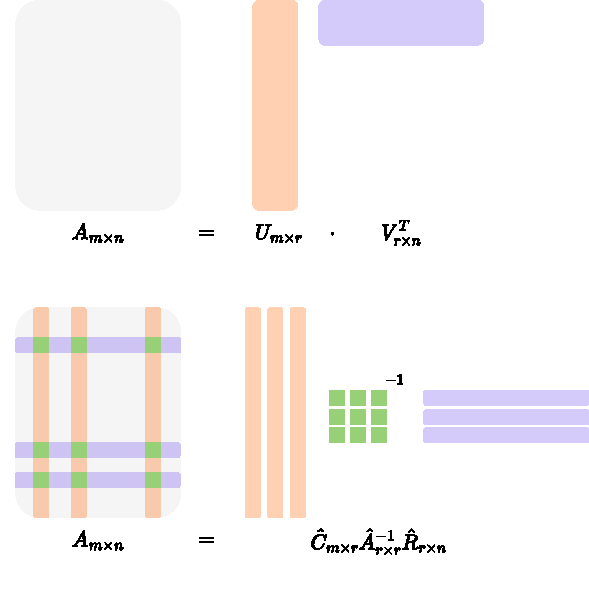
\includegraphics[keepaspectratio]{skeleton.pdf}}

}

\caption{\label{fig-skeleton}Иллюстрация рангового разложения}

\end{figure}%

\subsection{Каноническое тензорное
разложение}\label{ux43aux430ux43dux43eux43dux438ux447ux435ux441ux43aux43eux435-ux442ux435ux43dux437ux43eux440ux43dux43eux435-ux440ux430ux437ux43bux43eux436ux435ux43dux438ux435}

Можно рассмотреть обобщение рангового разложения на структуры данных
более высокого порядка, такие как тензоры, что означает представление
тензора в виде суммы \(r\) простых тензоров.

\begin{figure}[H]

{\centering 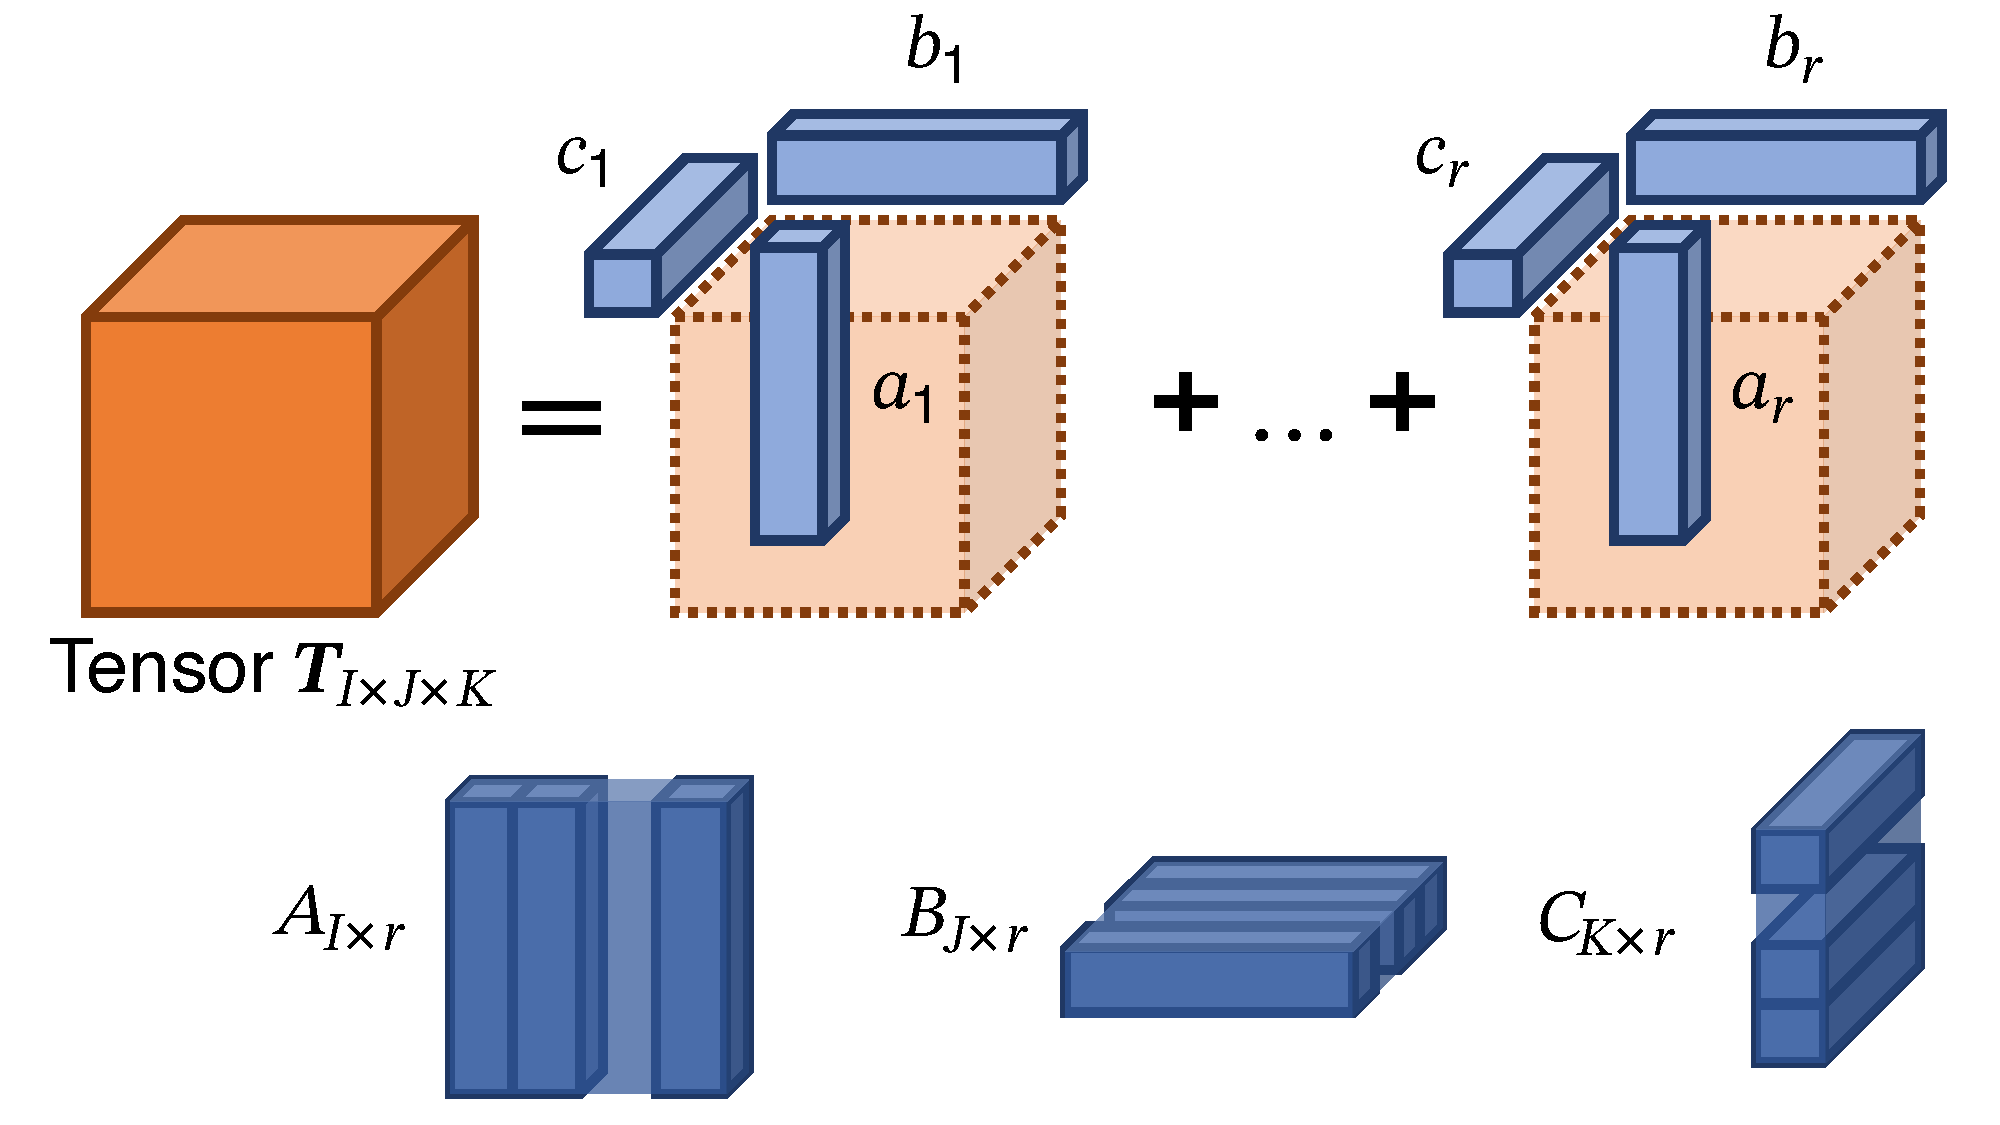
\includegraphics[width=0.4\linewidth,height=\textheight,keepaspectratio]{cp.pdf}

}

\caption{Иллюстрация канонического тензорного разложения}

\end{figure}%

\begin{tcolorbox}[enhanced jigsaw, breakable, toptitle=1mm, title=\textcolor{quarto-callout-color}{\faInfo}\hspace{0.5em}{Example}, colbacktitle=quarto-callout-color!10!white, opacityback=0, colback=white, left=2mm, coltitle=black, rightrule=.15mm, opacitybacktitle=0.6, colframe=quarto-callout-color-frame, bottomtitle=1mm, titlerule=0mm, arc=.35mm, bottomrule=.15mm, toprule=.15mm, leftrule=.75mm]

Заметьте, что существует множество тензорных разложений: каноническое,
Таккера, тензорный поезд (TT), тензорное кольцо (TR) и другие. В случае
тензоров мы не имеем прямого определения \emph{ранга} для всех типов
разложений. Например, для разложения Тензорного поезда ранг является не
скаляром, а вектором.

\end{tcolorbox}

\subsection{Определитель и след
матрицы}\label{ux43eux43fux440ux435ux434ux435ux43bux438ux442ux435ux43bux44c-ux438-ux441ux43bux435ux434-ux43cux430ux442ux440ux438ux446ux44b}

Определитель и след матрицы могут быть выражены через собственные
значения \[
\text{det} A = \prod\limits_{i=1}^n \lambda_i, \qquad \text{tr} A = \sum\limits_{i=1}^n \lambda_i
\] Определитель имеет несколько интересныхсвойств. Например,

\begin{itemize}
\tightlist
\item
  \(\text{det} A = 0\) тогда и только тогда, когда \(A\) является
  вырожденной;
\item
  \(\text{det}  AB = (\text{det} A)(\text{det}  B)\);
\item
  \(\text{det}  A^{-1} = \frac{1}{\text{det} \ A}\).
\end{itemize}

Не забывайте о циклическом свойстве следа для произвольных матриц
\(A, B, C, D\) (предполагая, что все размерности согласованы):

\[
\text{tr} (ABCD) = \text{tr} (DABC) = \text{tr} (CDAB) = \text{tr} (BCDA)
\]

\begin{tcolorbox}[enhanced jigsaw, breakable, toptitle=1mm, title=\textcolor{quarto-callout-color}{\faInfo}\hspace{0.5em}{Question}, colbacktitle=quarto-callout-color!10!white, opacityback=0, colback=white, left=2mm, coltitle=black, rightrule=.15mm, opacitybacktitle=0.6, colframe=quarto-callout-color-frame, bottomtitle=1mm, titlerule=0mm, arc=.35mm, bottomrule=.15mm, toprule=.15mm, leftrule=.75mm]

Как определитель матрицы связан с её обратимостью?

\end{tcolorbox}

\section{Скорости
сходимости}\label{ux441ux43aux43eux440ux43eux441ux442ux438-ux441ux445ux43eux434ux438ux43cux43eux441ux442ux438}

\subsection{Скорость
сходимости}\label{ux441ux43aux43eux440ux43eux441ux442ux44c-ux441ux445ux43eux434ux438ux43cux43eux441ux442ux438}

\begin{figure}[H]

{\centering \pandocbounded{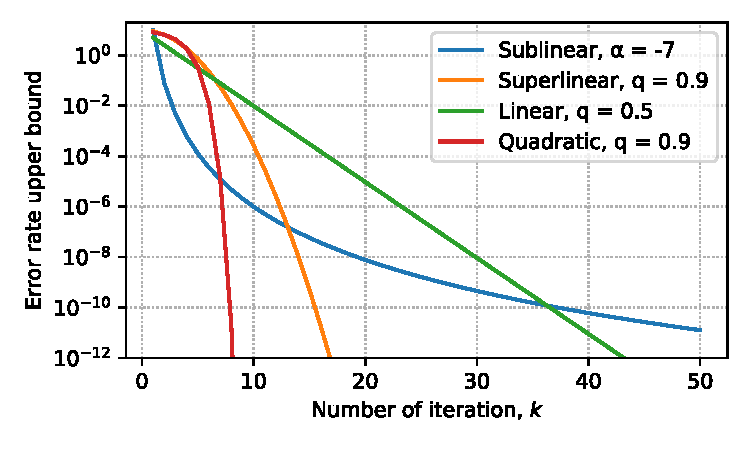
\includegraphics[keepaspectratio]{convergence.pdf}}

}

\caption{Разница в скоростях сходимости}

\end{figure}%

\subsection{Линейная
сходимость}\label{ux43bux438ux43dux435ux439ux43dux430ux44f-ux441ux445ux43eux434ux438ux43cux43eux441ux442ux44c}

Чтобы сравнить производительность алгоритмов, мы должны определить
термины для различных типов сходимости. Пусть \(r_k\) -
последовательность неотрицательных вещественных чисел, которая сходится
к нулю. Обычно мы имеем итерационный метод, который производит
последовательность итераций \(x_k\), приближающихся к оптимальному
решению \(x^*\), и \(r_k = \|x_k - x^*\|_2\).

\textbf{Линейная сходимость} последовательности \(r_k\) определяется
следующим образом:

Последовательность \(\{r_k\}_{k=m}^\infty\) сходится линейно с
параметром \(0 < q < 1\), если существует константа \(C > 0\) такая,
что: \[
r_k \leq C q^k, \quad \text{for all } k \geq m.
\] Если такое \(q\) существует, то последовательность называется линейно
сходящейся. \textbf{Точная нижняя граница} всех \(q\), удовлетворяющих
неравенству, называется \textbf{скоростью линейной сходимости}
последовательности.

\begin{tcolorbox}[enhanced jigsaw, breakable, toptitle=1mm, title=\textcolor{quarto-callout-color}{\faInfo}\hspace{0.5em}{Question}, colbacktitle=quarto-callout-color!10!white, opacityback=0, colback=white, left=2mm, coltitle=black, rightrule=.15mm, opacitybacktitle=0.6, colframe=quarto-callout-color-frame, bottomtitle=1mm, titlerule=0mm, arc=.35mm, bottomrule=.15mm, toprule=.15mm, leftrule=.75mm]

Предположим, у вас есть две последовательности с линейными скоростями
сходимости \(q_1 = 0.1\) и \(q_2 = 0.7\), какая из них быстрее?

\end{tcolorbox}

\subsection{Линейная
сходимость}\label{ux43bux438ux43dux435ux439ux43dux430ux44f-ux441ux445ux43eux434ux438ux43cux43eux441ux442ux44c-1}

\begin{tcolorbox}[enhanced jigsaw, breakable, toptitle=1mm, title=\textcolor{quarto-callout-color}{\faInfo}\hspace{0.5em}{Example}, colbacktitle=quarto-callout-color!10!white, opacityback=0, colback=white, left=2mm, coltitle=black, rightrule=.15mm, opacitybacktitle=0.6, colframe=quarto-callout-color-frame, bottomtitle=1mm, titlerule=0mm, arc=.35mm, bottomrule=.15mm, toprule=.15mm, leftrule=.75mm]

Предположим, у нас есть следующая последовательность:

\[
r_k = \dfrac{1}{2^k}
\]

Можно сразу заключить, что мы имеем линейную сходимость с параметрами
\(q = \dfrac{1}{2}\) и \(C = 0\).

\end{tcolorbox}

\begin{tcolorbox}[enhanced jigsaw, breakable, toptitle=1mm, title=\textcolor{quarto-callout-color}{\faInfo}\hspace{0.5em}{Question}, colbacktitle=quarto-callout-color!10!white, opacityback=0, colback=white, left=2mm, coltitle=black, rightrule=.15mm, opacitybacktitle=0.6, colframe=quarto-callout-color-frame, bottomtitle=1mm, titlerule=0mm, arc=.35mm, bottomrule=.15mm, toprule=.15mm, leftrule=.75mm]

Определите сходимость следующей последовательности \[
r_k = \dfrac{3}{2^k}
\]

\end{tcolorbox}

\subsection{Сублинейная
сходимость}\label{ux441ux443ux431ux43bux438ux43dux435ux439ux43dux430ux44f-ux441ux445ux43eux434ux438ux43cux43eux441ux442ux44c}

Если последовательность \(r_k\) сходится к нулю, но не имеет линейной
сходимости, то сходимость называется сублинейной. Иногда мы можем
рассмотреть следующий частный случай сублинейной сходимости: \[
\| x_{k+1} - x^* \|_2 \leq C k^{q},
\] где \(q < 0\) и \(0 < C < \infty\). Интуитивно, сублинейная
сходимость означает, что последовательность сходится медленнее любой
геометрической прогрессии.

\subsection{Сверхлинейная
сходимость}\label{ux441ux432ux435ux440ux445ux43bux438ux43dux435ux439ux43dux430ux44f-ux441ux445ux43eux434ux438ux43cux43eux441ux442ux44c}

Сходимость последовательности \(\{r_k\}_{k=m}^\infty\) называется
\textbf{сверхлинейной}, если она сходится к нулю быстрее любой линейно
сходящейся последовательности. Проверьте, что последовательность
\(\{r_k\}_{k=m}^\infty\) является сверхлинейной, если она сходится
линейно с параметром \(q = 0\).

Для \(p > 1\), последовательность имеет \textbf{сверхлинейную сходимость
порядка \(p\)}, если существует \(C > 0\) и \(0 < q < 1\) такая, что: \[
r_k \leq C q^{p^k}, \quad \text{for all } k \geq m.
\] Когда \(p = 2\), это называется \textbf{квадратичной сходимостью}.

\begin{tcolorbox}[enhanced jigsaw, breakable, toptitle=1mm, title=\textcolor{quarto-callout-color}{\faInfo}\hspace{0.5em}{Важный пример}, colbacktitle=quarto-callout-color!10!white, opacityback=0, colback=white, left=2mm, coltitle=black, rightrule=.15mm, opacitybacktitle=0.6, colframe=quarto-callout-color-frame, bottomtitle=1mm, titlerule=0mm, arc=.35mm, bottomrule=.15mm, toprule=.15mm, leftrule=.75mm]

Предположим, что \(x^* = 1.23456789\) (истинное решение), и итерационная
последовательность начинается с ошибки \(r_k = 10^{-3}\),
соответствующей 3 правильным значащим цифрам (\(1.234\)).

\begin{enumerate}
\def\labelenumi{\arabic{enumi}.}
\item
  После первой итерации: \[
  r_{k+1} \approx r_k^2 = (10^{-3})^2 = 10^{-6}.
  \] Теперь ошибка равна \(10^{-6}\), и мы имеем 6 правильных значащих
  цифр (\(1.23456\)).
\item
  После второй итерации: \[
  r_{k+2} \approx r_{k+1}^2 = (10^{-6})^2 = 10^{-12}.
  \] Теперь ошибка равна \(10^{-12}\), и мы имеем 12 правильных значащих
  цифр (\(1.234567890123\)).
\end{enumerate}

\end{tcolorbox}

\subsection{Практические наблюдения о скоростях
сходимости}\label{ux43fux440ux430ux43aux442ux438ux447ux435ux441ux43aux438ux435-ux43dux430ux431ux43bux44eux434ux435ux43dux438ux44f-ux43e-ux441ux43aux43eux440ux43eux441ux442ux44fux445-ux441ux445ux43eux434ux438ux43cux43eux441ux442ux438}

\begin{itemize}
\tightlist
\item
  \(\|x_{k+1} - x^*\|_2 \leq \frac{1}{k^{\frac1p}} \|x_0 - x^*\|_2\)
  означает сублинейную скорость сходимости
\item
  \(\|x_{k+1} - x^*\|_2 \leq q \|x_k - x^*\|_2\) означает линейную
  скорость сходимости, где \(q<1\)
\item
  \(\|x_{k+1} - x^*\|_2 \leq q \|x_k - x^*\|_2^2\) означает квадратичную
  скорость сходимости, где \(q\|x_0 - x^*\|<1\)
\end{itemize}

\subsection{Тест
корней}\label{ux442ux435ux441ux442-ux43aux43eux440ux43dux435ux439}

\begin{tcolorbox}[enhanced jigsaw, breakable, toptitle=1mm, title=\textcolor{quarto-callout-color}{\faInfo}\hspace{0.5em}{Theorem}, colbacktitle=quarto-callout-color!10!white, opacityback=0, colback=white, left=2mm, coltitle=black, rightrule=.15mm, opacitybacktitle=0.6, colframe=quarto-callout-color-frame, bottomtitle=1mm, titlerule=0mm, arc=.35mm, bottomrule=.15mm, toprule=.15mm, leftrule=.75mm]

Пусть \((r_k)_{k=m}^\infty\) - последовательность неотрицательных чисел,
сходящаяся к нулю, и пусть
\(\alpha := \limsup_{k \to \infty} r_k^{1/k}\). (Заметим, что
\(\alpha \geq 0\).)

\begin{enumerate}
\def\labelenumi{(\alph{enumi})}
\item
  Если \(0 \leq \alpha < 1\), то \((r_k)_{k=m}^\infty\) сходится линейно
  с константой \(\alpha\).
\item
  В частности, если \(\alpha = 0\), то \((r_k)_{k=m}^\infty\) сходится
  сверхлинейно.
\item
  Если \(\alpha = 1\), то \((r_k)_{k=m}^\infty\) сходится сублинейно.
\item
  Случай \(\alpha > 1\) невозможен.
\end{enumerate}

\textbf{Доказательство}.

\begin{enumerate}
\def\labelenumi{\arabic{enumi}.}
\item
  Покажем, что если \((r_k)_{k=m}^\infty\) сходится линейно с константой
  \(0 \leq \beta < 1\), то \(\alpha \leq \beta\). Действительно, по
  определению константы линейной сходимости, для любого
  \(\varepsilon > 0\) такого, что \(\beta + \varepsilon < 1\),
  существует \(C > 0\) такое, что \(r_k \leq C(\beta + \varepsilon)^k\)
  для всех \(k \geq m\). Отсюда,
  \(r_k^{1/k} \leq C^{1/k}(\beta + \varepsilon)\) для всех \(k \geq m\).
  Переходя к пределу при \(k \to \infty\) и используя \(C^{1/k} \to 1\),
  мы получаем \(\alpha \leq \beta + \varepsilon\). Учитывая
  произвольность \(\varepsilon\), получаем \(\alpha \leq \beta\).
\item
  Таким образом, в случае \(\alpha = 1\) последовательность
  \((r_k)_{k=m}^\infty\) не может иметь линейной сходимости в
  соответствии с приведенным выше результатом (доказано от противного).
  Тем не менее, \((r_k)_{k=m}^\infty\) сходится к нулю, поэтому она
  должна сходиться сублинейно.
\end{enumerate}

\end{tcolorbox}

\subsection{Тест
корней}\label{ux442ux435ux441ux442-ux43aux43eux440ux43dux435ux439-1}

\begin{tcolorbox}[enhanced jigsaw, breakable, toptitle=1mm, title=\textcolor{quarto-callout-color}{\faInfo}\hspace{0.5em}{Theorem}, colbacktitle=quarto-callout-color!10!white, opacityback=0, colback=white, left=2mm, coltitle=black, rightrule=.15mm, opacitybacktitle=0.6, colframe=quarto-callout-color-frame, bottomtitle=1mm, titlerule=0mm, arc=.35mm, bottomrule=.15mm, toprule=.15mm, leftrule=.75mm]

\begin{enumerate}
\def\labelenumi{\arabic{enumi}.}
\item
  Теперь рассмотрим случай \(0 \leq \alpha < 1\). Пусть
  \(\varepsilon > 0\) - произвольное число такое, что
  \(\alpha + \varepsilon < 1\). Согласно свойствам limsup, существует
  \(N \geq m\) такое, что \(r_k^{1/k} \leq \alpha + \varepsilon\) для
  всех \(k \geq N\). Отсюда, \(r_k \leq (\alpha + \varepsilon)^k\) для
  всех \(k \geq N\). Следовательно, \((r_k)_{k=m}^\infty\) сходится
  линейно с параметром \(\alpha + \varepsilon\) (не имеет значения, что
  неравенство выполняется только для числа \(N\)). Учитывая
  произвольность \(\varepsilon\), это означает, что константа линейной
  сходимости \((r_k)_{k=m}^\infty\) не превышает \(\alpha\). Поскольку,
  как показано выше, константа линейной сходимости не может быть меньше
  \(\alpha\), это означает, что константа линейной сходимости
  \((r_k)_{k=m}^\infty\) точно равна \(\alpha\).
\item
  Наконец, покажем, что случай \(\alpha > 1\) невозможен. Действительно,
  предположим, что \(\alpha > 1\). Тогда из определения limsup следует,
  что для любого \(N \geq m\) существует \(k \geq N\) такое, что
  \(r_k^{1/k} \geq 1\), и, в частности, \(r_k \geq 1\). Но это означает,
  что \(r_k\) имеет подпоследовательность, которая не ограничена от
  нуля. Следовательно, \((r_k)_{k=m}^\infty\) не может сходиться к нулю,
  что противоречит условию.
\end{enumerate}

\end{tcolorbox}

\subsection{Тест
отношений}\label{ux442ux435ux441ux442-ux43eux442ux43dux43eux448ux435ux43dux438ux439}

Пусть \(\{r_k\}_{k=m}^\infty\) - последовательность строго положительных
чисел, сходящаяся к нулю. Пусть

\[
q = \lim_{k \to \infty} \dfrac{r_{k+1}}{r_k}
\]

\begin{itemize}
\tightlist
\item
  Если существует \(q\) и \(0 \leq q <  1\), то \(\{r_k\}_{k=m}^\infty\)
  имеет линейную сходимость с константой \(q\).
\item
  В частности, если \(q = 0\), то \(\{r_k\}_{k=m}^\infty\) имеет
  сверхлинейную сходимость.
\item
  Если \(q\) не существует, но
  \(q = \lim\limits_{k \to \infty} \sup_k \dfrac{r_{k+1}}{r_k} <  1\),
  то \(\{r_k\}_{k=m}^\infty\) имеет линейную сходимость с константой, не
  превышающей \(q\).
\item
  Если \(\lim\limits_{k \to \infty} \inf_k \dfrac{r_{k+1}}{r_k} =1\), то
  \(\{r_k\}_{k=m}^\infty\) имеет сублинейную сходимость.
\item
  Случай \(\lim\limits_{k \to \infty} \inf_k \dfrac{r_{k+1}}{r_k} > 1\)
  невозможен.
\item
  В остальных случаях (т.е., когда
  \(\lim\limits_{k \to \infty} \inf_k \dfrac{r_{k+1}}{r_k} <  1 \leq  \lim\limits_{k \to \infty} \sup_k \dfrac{r_{k+1}}{r_k}\))
  мы не можем сделать никаких конкретных утверждений о скорости
  сходимости \(\{r_k\}_{k=m}^\infty\).
\end{itemize}

\subsection{Лемма о тесте
отношений}\label{ux43bux435ux43cux43cux430-ux43e-ux442ux435ux441ux442ux435-ux43eux442ux43dux43eux448ux435ux43dux438ux439}

\begin{tcolorbox}[enhanced jigsaw, breakable, toptitle=1mm, title=\textcolor{quarto-callout-color}{\faInfo}\hspace{0.5em}{Theorem}, colbacktitle=quarto-callout-color!10!white, opacityback=0, colback=white, left=2mm, coltitle=black, rightrule=.15mm, opacitybacktitle=0.6, colframe=quarto-callout-color-frame, bottomtitle=1mm, titlerule=0mm, arc=.35mm, bottomrule=.15mm, toprule=.15mm, leftrule=.75mm]

Пусть \((r_k)_{k=m}^\infty\) - последовательность строго положительных
чисел. (Строгая положительность необходима для того, чтобы отношения
\(\frac{r_{k+1}}{r_k}\), которые появляются ниже, были определены.)
Тогда

\[
\liminf_{k \to \infty} \frac{r_{k+1}}{r_k} \leq \liminf_{k \to \infty} r_k^{1/k} \leq \limsup_{k \to \infty} r_k^{1/k} \leq \limsup_{k \to \infty} \frac{r_{k+1}}{r_k}.
\]

\textbf{Доказательство}.

\begin{enumerate}
\def\labelenumi{\arabic{enumi}.}
\item
  Среднее неравенство следует из того, что liminf любой
  последовательности всегда меньше или равен её limsup. Докажем
  последнее неравенство; первое доказывается аналогично.
\item
  Обозначим \(L := \limsup_{k \to \infty} \frac{r_{k+1}}{r_k}\). Если
  \(L = +\infty\), то неравенство очевидно, поэтому предположим, что
  \(L\) конечно. Заметим, что \(L \geq 0\), поскольку отношение
  \(\frac{r_{k+1}}{r_k}\) положительно для всех \(k \geq m\). Пусть
  \(\varepsilon > 0\) - произвольное число. Согласно свойствам limsup,
  существует \(N \geq m\) такое, что
  \(\frac{r_{k+1}}{r_k} \leq L + \varepsilon\) для всех \(k \geq N\).
  Отсюда, \(r_{k+1} \leq (L + \varepsilon)r_k\) для всех \(k \geq N\).
  Применяя индукцию, получаем \(r_k \leq (L + \varepsilon)^{k-N}r_N\)
  для всех \(k \geq N\). Пусть \(C := (L + \varepsilon)^{-N}r_N\). Тогда
  \(r_k \leq C(L + \varepsilon)^k\) для всех \(k \geq N\), откуда
  \(r_k^{1/k} \leq C^{1/k}(L + \varepsilon)\). Переходя к limsup при
  \(k \to \infty\) и используя \(C^{1/k} \to 1\), получаем
  \(\limsup_{k \to \infty} r_k^{1/k} \leq L + \varepsilon\). Учитывая
  произвольность \(\varepsilon\), получаем
  \(\limsup_{k \to \infty} r_k^{1/k} \leq L\).
\end{enumerate}

\end{tcolorbox}

\section{Задачи}\label{ux437ux430ux434ux430ux447ux438}

\subsection{Задача 1. Простая, но важная идея о матричных
вычислениях.}\label{ux437ux430ux434ux430ux447ux430-1.-ux43fux440ux43eux441ux442ux430ux44f-ux43dux43e-ux432ux430ux436ux43dux430ux44f-ux438ux434ux435ux44f-ux43e-ux43cux430ux442ux440ux438ux447ux43dux44bux445-ux432ux44bux447ux438ux441ux43bux435ux43dux438ux44fux445.}

Предположим, у вас есть следующее выражение

\[
b = A_1 A_2 A_3 x,
\]

где \(A_1, A_2, A_3 \in \mathbb{R}^{3 \times 3}\) - случайные квадратные
плотные матрицы, и \(x \in \mathbb{R}^n\) - вектор. Вам нужно вычислить
\(b\).

Какой способ лучше всего использовать?

\begin{enumerate}
\def\labelenumi{\arabic{enumi}.}
\tightlist
\item
  \(A_1 A_2 A_3 x\) (слева направо)
\item
  \(\left(A_1 \left(A_2 \left(A_3 x\right)\right)\right)\) (справа
  налево)
\item
  Не имеет значения
\item
  Результаты первых двух вариантов не будут одинаковыми.
\end{enumerate}

Проверьте простой
\href{https://colab.research.google.com/github/MerkulovDaniil/optim/blob/master/assets/Notebooks/stupid_important_idea_on_mm.ipynb}{\faPython~код}
после вашего интуитивного ответа.

\subsection{Задача 2. Связь между Фробениусовой нормой и сингулярными
значениями.}\label{ux437ux430ux434ux430ux447ux430-2.-ux441ux432ux44fux437ux44c-ux43cux435ux436ux434ux443-ux444ux440ux43eux431ux435ux43dux438ux443ux441ux43eux432ux43eux439-ux43dux43eux440ux43cux43eux439-ux438-ux441ux438ux43dux433ux443ux43bux44fux440ux43dux44bux43cux438-ux437ux43dux430ux447ux435ux43dux438ux44fux43cux438.}

Пусть \(A \in \mathbb{R}^{m \times n}\), и пусть \(q := \min\{m, n\}\).
Докажите, что \[
\|A\|_F^2 = \sum_{i=1}^{q} \sigma_i^2(A) ,
\]

где \(\sigma_1(A) \geq \ldots \geq \sigma_q(A) \geq 0\) - сингулярные
значения матрицы \(A\). Подсказка: используйте связь между Фробениусовой
нормой и скалярным произведением и SVD.

\subsection{Задача 3. Знайте свое скалярное
произведение.}\label{ux437ux430ux434ux430ux447ux430-3.-ux437ux43dux430ux439ux442ux435-ux441ux432ux43eux435-ux441ux43aux430ux43bux44fux440ux43dux43eux435-ux43fux440ux43eux438ux437ux432ux435ux434ux435ux43dux438ux435.}

Упростите следующее выражение:

\[
\sum\limits_{i=1}^n \langle S^{-1} a_i, a_i \rangle,
\] где
\(S = \sum\limits_{i=1}^n a_ia_i^T, a_i \in \mathbb{R}^n, \det(S) \neq 0\)

\subsection{Задача 4. Простые скорости
сходимости.}\label{ux437ux430ux434ux430ux447ux430-4.-ux43fux440ux43eux441ux442ux44bux435-ux441ux43aux43eux440ux43eux441ux442ux438-ux441ux445ux43eux434ux438ux43cux43eux441ux442ux438.}

Определите сходимость (и её скорость) или расходимость следующих
последовательностей:

\begin{itemize}
\tightlist
\item
  \(r_{k} = \frac{1}{3^k}\)
\item
  \(r_{k} = \frac{4}{3^k}\)
\item
  \(r_{k} = \frac{1}{k^{10}}\)
\item
  \(r_{k} = 0.707^k\)
\item
  \(r_{k} = 0.707^{2^k}\)
\end{itemize}

\subsection{Задача 5. Один тест проще, чем
другой.}\label{ux437ux430ux434ux430ux447ux430-5.-ux43eux434ux438ux43d-ux442ux435ux441ux442-ux43fux440ux43eux449ux435-ux447ux435ux43c-ux434ux440ux443ux433ux43eux439.}

Определите сходимость (и её скорость) или расходимость следующей
последовательности:

\[
r_{k} = \frac{1}{k^k}
\]

\subsection{Задача 6. Сверхлинейно, но не
квадратично.}\label{ux437ux430ux434ux430ux447ux430-6.-ux441ux432ux435ux440ux445ux43bux438ux43dux435ux439ux43dux43e-ux43dux43e-ux43dux435-ux43aux432ux430ux434ux440ux430ux442ux438ux447ux43dux43e.}

Покажите, что следующая последовательность не имеет квадратичной
сходимости.

\[
r_{k} = \frac{1}{3^{k^2}}
\]

\section{А где это нужно в реальной
жизни?}\label{ux430-ux433ux434ux435-ux44dux442ux43e-ux43dux443ux436ux43dux43e-ux432-ux440ux435ux430ux43bux44cux43dux43eux439-ux436ux438ux437ux43dux438}

\subsection{\texorpdfstring{LoRA: Low-Rank Adaptation of Large Language
Models
(\href{https://arxiv.org/pdf/2106.09685}{arXiv:2106.09685})}{LoRA: Low-Rank Adaptation of Large Language Models (arXiv:2106.09685)}}\label{lora-low-rank-adaptation-of-large-language-models-arxiv2106.09685}

Поскольку современные LLM слишком большие, чтобы вместиться в память
среднего пользователя, мы используем некоторые трюки, чтобы сделать их
потребление памяти меньше. Одним из наиболее популярных трюков является
LoRA (Low-Rank Adaptation of Large Language Models).

Предположим, у нас есть матрица \(W \in \mathbb{R}^{d \times k}\) и мы
хотим выполнить следующее обновление: \[
W = W_0 + \Delta W.
\] Основная идея LoRA состоит в том, чтобы разложить обновление
\(\Delta W\) на две низкоранговые матрицы:

\begin{gather*}
W = W_0 + \Delta W = W_0 + BA, \quad B \in \mathbb{R}^{d \times r}, A \in \mathbb{R}^{r \times k}, \\
rank(A) = rank(B) = r \ll \min\{d, k\}.
\end{gather*}

Проверьте
\href{https://colab.research.google.com/github/MerkulovDaniil/hse25/blob/main/notebooks/s1_lora_trump.ipynb}{\faPython~ноутбук}
для примера реализации LoRA.

\begin{figure}[H]

{\centering 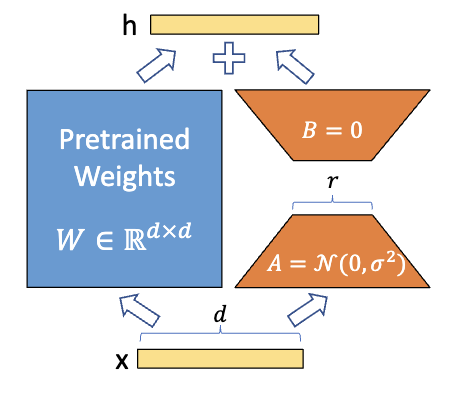
\includegraphics[width=1\linewidth,height=\textheight,keepaspectratio]{lora.png}

}

\caption{Иллюстрация LoRA}

\end{figure}%

\section{Задачи на
дом}\label{ux437ux430ux434ux430ux447ux438-ux43dux430-ux434ux43eux43c}

\subsubsection{Вспоминаем линейную
алгебру}\label{ux432ux441ux43fux43eux43cux438ux43dux430ux435ux43c-ux43bux438ux43dux435ux439ux43dux443ux44e-ux430ux43bux433ux435ux431ux440ux443-1}

\begin{enumerate}
\def\labelenumi{\arabic{enumi}.}
\item
  {[}5 points{]} \textbf{Анализ чувствительности в линейных системах}
  Рассмотрим невырожденную матрицу \(A \in \mathbb{R}^{n \times n}\) и
  вектор \(b \in \mathbb{R}^n\). Предположим, что из-за ошибок измерения
  или вычислений вектор \(b\) изменяется на
  \(\tilde{b} = b + \delta b\).

  \begin{enumerate}
  \def\labelenumii{\arabic{enumii}.}
  \tightlist
  \item
    Выведите верхнюю оценку относительной ошибки в решении \(x\) системы
    \(Ax = b\) в терминах числа обусловленности \(\kappa(A)\) и
    относительной ошибки в \(b\).\\
  \item
    Приведите конкретный пример использования матрицы \(2 \times 2\),
    где \(\kappa(A)\) велико (например, \(\geq 100500\)).
  \end{enumerate}
\item
  {[}5 points{]} \textbf{Влияние диагонального масштабирования на ранг}
  Пусть \(A \in \mathbb{R}^{n \times n}\) - матрица ранга \(r\). Пусть
  \(D \in \mathbb{R}^{n \times n}\) - диагональная матрица. Определите
  ранг произведения \(DA\). Объясните ваше обоснование.
\item
  {[}8 points{]} \textbf{Неожиданный SVD} Вычислите сингулярное
  разложение (SVD) следующих матриц:

  \begin{itemize}
  \tightlist
  \item
    \(A_1 = \begin{bmatrix} 2 \\ 2 \\ 8 \end{bmatrix}\)
  \item
    \(A_2 = \begin{bmatrix} 0 & x \\ x & 0 \\ 0 & 0 \end{bmatrix}\), где
    \(x\) - сумма чисел вашего рождения (день + месяц).
  \end{itemize}
\item
  {[}10 points{]} \textbf{Влияние нормализации на ранг} Предположим, у
  нас есть набор данных \(x^{(i)}\in\mathbb{R}^{n},\,i=1,\dots,m\), и мы
  решили представить эти данные в виде матрицы \[
   X =
   \begin{pmatrix}
    | & & | \\
    x^{(1)} & \dots & x^{(m)} \\
    | & & | \\
   \end{pmatrix} \in \mathbb{R}^{n \times m}.
   \]

  Предположим, что \(\text{rank}\,X = r\).

  В следующей задаче мы просим вас найти ранг некоторой матрицы \(M\),
  связанной с \(X\). В частности, вам нужно найти связь между
  \(\text{rank}\,X = r\) и \(\text{rank}\,M\), например, что ранг \(M\)
  всегда больше/меньше ранга \(X\) или что
  \(\text{rank}\,M = \text{rank}\,X \big / 35\). Аргументируйте ваш
  ответ и сделайте его как можно более точным.

  Обратите внимание, что граничные случаи возможны в зависимости от
  структуры матрицы \(X\). Убедитесь, что вы правильно освещаете их в
  своем ответе.

  В прикладной статистике и машинном обучении данные часто
  нормализуются. Одна из наиболее популярных стратегий состоит в том,
  чтобы вычесть оцененное среднее \(\mu\) и разделить на квадратный
  корень из оцененной дисперсии \(\sigma^2\). т.е. \[
   x \rightarrow (x - \mu) \big / \sigma.
   \] После нормализации мы получаем новую матрицу \[
   \begin{split}
   Y &:=
   \begin{pmatrix}
    | & & | \\
    y^{(1)} & \dots & y^{(m)} \\
    | & & | \\
   \end{pmatrix},\\
   y^{(i)} &:= \frac{x^{(i)} - \frac{1}{m}\sum_{j=1}^{m} x^{(j)}}{\sigma}.
   \end{split}
   \] Каков ранг \(Y\) если \(\text{rank} \; X = r\)? Здесь \(\sigma\) -
  вектор, и деление выполняется поэлементно. Причина этого в том, что
  разные признаки могут иметь разные масштабы. В частности: \[
   \sigma_i = \sqrt{\frac{1}{m}\sum_{j=1}^{m} \left(x_i^{(j)}\right)^2 - \left(\frac{1}{m}\sum_{j=1}^{m} x_i^{(j)}\right)^2}.
   \]
\item
  {[}20 points{]} \textbf{Сжатие изображений с использованием усеченного
  SVD} Исследуйте сжатие изображений с использованием усеченного
  сингулярного разложения (SVD). Понимание того, как изменение
  количества сингулярных значений влияет на качество сжатого
  изображения. Реализуйте Python скрипт для сжатия черно-белого
  изображения с использованием усеченного SVD и визуализируйте качество
  сжатия.

  \begin{itemize}
  \tightlist
  \item
    \textbf{Усеченное SVD}: Разлагает изображение \(A\) на матрицы
    \(U, S,\) и \(V\). Сжатое изображение восстанавливается с
    использованием подмножества сингулярных значений.
  \item
    \textbf{Математическое представление}: \[
      A \approx U_k \Sigma_k V_k^T
      \]

    \begin{itemize}
    \tightlist
    \item
      \(U_k\) и \(V_k\) - первые \(k\) столбцов \(U\) и \(V\)
      соответственно.
    \item
      \(\Sigma_k\) - диагональная матрица с первыми \(k\) сингулярными
      значениями.
    \item
      \textbf{Относительная ошибка}: Измеряет точность сжатого
      изображения по сравнению с оригиналом. \[
        \text{Relative Error} = \frac{\| A - A_k \|}{\| A \|}
        \]
    \end{itemize}
  \end{itemize}

\begin{Shaded}
\begin{Highlighting}[]
\ImportTok{import}\NormalTok{ matplotlib.pyplot }\ImportTok{as}\NormalTok{ plt}
\ImportTok{import}\NormalTok{ matplotlib.animation }\ImportTok{as}\NormalTok{ animation}
\ImportTok{import}\NormalTok{ numpy }\ImportTok{as}\NormalTok{ np}
\ImportTok{from}\NormalTok{ skimage }\ImportTok{import}\NormalTok{ io, color}
\ImportTok{import}\NormalTok{ requests}
\ImportTok{from}\NormalTok{ io }\ImportTok{import}\NormalTok{ BytesIO}

\KeywordTok{def}\NormalTok{ download\_image(url):}
\NormalTok{    response }\OperatorTok{=}\NormalTok{ requests.get(url)}
\NormalTok{    img }\OperatorTok{=}\NormalTok{ io.imread(BytesIO(response.content))}
    \ControlFlowTok{return}\NormalTok{ color.rgb2gray(img)  }\CommentTok{\# Convert to grayscale}

\KeywordTok{def}\NormalTok{ update\_plot(i, img\_plot, error\_plot, U, S, V, original\_img, errors, ranks, ax1, ax2):}
    \CommentTok{\# Adjust rank based on the frame index}
    \ControlFlowTok{if}\NormalTok{ i }\OperatorTok{\textless{}} \DecValTok{70}\NormalTok{:}
\NormalTok{        rank }\OperatorTok{=}\NormalTok{ i }\OperatorTok{+} \DecValTok{1}
    \ControlFlowTok{else}\NormalTok{:}
\NormalTok{        rank }\OperatorTok{=} \DecValTok{70} \OperatorTok{+}\NormalTok{ (i }\OperatorTok{{-}} \DecValTok{69}\NormalTok{) }\OperatorTok{*} \DecValTok{10}

\NormalTok{    reconstructed\_img }\OperatorTok{=}\NormalTok{ ... }\CommentTok{\# YOUR CODE HERE }

    \CommentTok{\# Calculate relative error}
\NormalTok{    relative\_error }\OperatorTok{=}\NormalTok{ ... }\CommentTok{\# YOUR CODE HERE}
\NormalTok{    errors.append(relative\_error)}
\NormalTok{    ranks.append(rank)}

    \CommentTok{\# Update the image plot and title}
\NormalTok{    img\_plot.set\_data(reconstructed\_img)}
\NormalTok{    ax1.set\_title(}\SpecialStringTok{f"Image compression with SVD}\CharTok{\textbackslash{}n}\SpecialStringTok{ Rank }\SpecialCharTok{\{}\NormalTok{rank}\SpecialCharTok{\}}\SpecialStringTok{; Relative error }\SpecialCharTok{\{}\NormalTok{relative\_error}\SpecialCharTok{:.2f\}}\SpecialStringTok{"}\NormalTok{)}

    \CommentTok{\# Remove axis ticks and labels from the first subplot (ax1)}
\NormalTok{    ax1.set\_xticks([])}
\NormalTok{    ax1.set\_yticks([])}

    \CommentTok{\# Update the error plot}
\NormalTok{    error\_plot.set\_data(ranks, errors)}
\NormalTok{    ax2.set\_xlim(}\DecValTok{1}\NormalTok{, }\BuiltInTok{len}\NormalTok{(S))}
\NormalTok{    ax2.grid(linestyle}\OperatorTok{=}\StringTok{":"}\NormalTok{)}
\NormalTok{    ax2.set\_ylim(}\FloatTok{1e{-}4}\NormalTok{, }\FloatTok{0.5}\NormalTok{)}
\NormalTok{    ax2.set\_ylabel(}\StringTok{\textquotesingle{}Relative Error\textquotesingle{}}\NormalTok{)}
\NormalTok{    ax2.set\_xlabel(}\StringTok{\textquotesingle{}Rank\textquotesingle{}}\NormalTok{)}
\NormalTok{    ax2.set\_title(}\StringTok{\textquotesingle{}Relative Error over Rank\textquotesingle{}}\NormalTok{)}
\NormalTok{    ax2.semilogy()}

    \CommentTok{\# Set xticks to show rank numbers}
\NormalTok{    ax2.set\_xticks(}\BuiltInTok{range}\NormalTok{(}\DecValTok{1}\NormalTok{, }\BuiltInTok{len}\NormalTok{(S)}\OperatorTok{+}\DecValTok{1}\NormalTok{, }\BuiltInTok{max}\NormalTok{(}\BuiltInTok{len}\NormalTok{(S)}\OperatorTok{//}\DecValTok{10}\NormalTok{, }\DecValTok{1}\NormalTok{)))  }\CommentTok{\# Adjust the step size as needed}
\NormalTok{    plt.tight\_layout()}

    \ControlFlowTok{return}\NormalTok{ img\_plot, error\_plot}


\KeywordTok{def}\NormalTok{ create\_animation(image, filename}\OperatorTok{=}\StringTok{\textquotesingle{}svd\_animation.mp4\textquotesingle{}}\NormalTok{):}
\NormalTok{    U, S, V }\OperatorTok{=}\NormalTok{ np.linalg.svd(image, full\_matrices}\OperatorTok{=}\VariableTok{False}\NormalTok{)}
\NormalTok{    errors }\OperatorTok{=}\NormalTok{ []}
\NormalTok{    ranks }\OperatorTok{=}\NormalTok{ []}

\NormalTok{    fig, (ax1, ax2) }\OperatorTok{=}\NormalTok{ plt.subplots(}\DecValTok{2}\NormalTok{, }\DecValTok{1}\NormalTok{, figsize}\OperatorTok{=}\NormalTok{(}\DecValTok{5}\NormalTok{, }\DecValTok{8}\NormalTok{))}
\NormalTok{    img\_plot }\OperatorTok{=}\NormalTok{ ax1.imshow(image, cmap}\OperatorTok{=}\StringTok{\textquotesingle{}gray\textquotesingle{}}\NormalTok{, animated}\OperatorTok{=}\VariableTok{True}\NormalTok{)}
\NormalTok{    error\_plot, }\OperatorTok{=}\NormalTok{ ax2.plot([], [], }\StringTok{\textquotesingle{}r{-}\textquotesingle{}}\NormalTok{, animated}\OperatorTok{=}\VariableTok{True}\NormalTok{)  }\CommentTok{\# Initial empty plot for errors}

    \CommentTok{\# Add watermark}
\NormalTok{    ax1.text(}\DecValTok{1}\NormalTok{, }\FloatTok{1.02}\NormalTok{, }\StringTok{\textquotesingle{}@fminxyz\textquotesingle{}}\NormalTok{, transform}\OperatorTok{=}\NormalTok{ax1.transAxes, color}\OperatorTok{=}\StringTok{\textquotesingle{}gray\textquotesingle{}}\NormalTok{, va}\OperatorTok{=}\StringTok{\textquotesingle{}bottom\textquotesingle{}}\NormalTok{, ha}\OperatorTok{=}\StringTok{\textquotesingle{}right\textquotesingle{}}\NormalTok{, fontsize}\OperatorTok{=}\DecValTok{9}\NormalTok{)}

    \CommentTok{\# Determine frames for the animation}
\NormalTok{    initial\_frames }\OperatorTok{=} \BuiltInTok{list}\NormalTok{(}\BuiltInTok{range}\NormalTok{(}\DecValTok{70}\NormalTok{))  }\CommentTok{\# First 70 ranks}
\NormalTok{    subsequent\_frames }\OperatorTok{=} \BuiltInTok{list}\NormalTok{(}\BuiltInTok{range}\NormalTok{(}\DecValTok{70}\NormalTok{, }\BuiltInTok{len}\NormalTok{(S), }\DecValTok{10}\NormalTok{))  }\CommentTok{\# Every 10th rank after 70}
\NormalTok{    frames }\OperatorTok{=}\NormalTok{ initial\_frames }\OperatorTok{+}\NormalTok{ subsequent\_frames}

\NormalTok{    ani }\OperatorTok{=}\NormalTok{ animation.FuncAnimation(fig, update\_plot, frames}\OperatorTok{=}\BuiltInTok{len}\NormalTok{(frames), fargs}\OperatorTok{=}\NormalTok{(img\_plot, error\_plot, U, S, V, image, errors, ranks, ax1, ax2), interval}\OperatorTok{=}\DecValTok{50}\NormalTok{, blit}\OperatorTok{=}\VariableTok{True}\NormalTok{)}
\NormalTok{    ani.save(filename, writer}\OperatorTok{=}\StringTok{\textquotesingle{}ffmpeg\textquotesingle{}}\NormalTok{, fps}\OperatorTok{=}\DecValTok{8}\NormalTok{, dpi}\OperatorTok{=}\DecValTok{300}\NormalTok{)}

    \CommentTok{\# URL of the image}
\NormalTok{    url }\OperatorTok{=} \StringTok{""}

    \CommentTok{\# Download the image and create the animation}
\NormalTok{    image }\OperatorTok{=}\NormalTok{ download\_image(url)}
\NormalTok{    create\_animation(image)}
\end{Highlighting}
\end{Shaded}
\end{enumerate}

\subsubsection{Скорости
сходимости}\label{ux441ux43aux43eux440ux43eux441ux442ux438-ux441ux445ux43eux434ux438ux43cux43eux441ux442ux438-1}

\begin{enumerate}
\def\labelenumi{\arabic{enumi}.}
\item
  {[}6 points{]} Определите (это означает определить характер
  сходимости, если она сходится) сходимость или расходимость следующих
  последовательностей

  \begin{itemize}
  \tightlist
  \item
    \(r_{k} = \frac{1}{\sqrt{k+5}}\).
  \item
    \(r_{k} = 0.101^k\).
  \item
    \(r_{k} = 0.101^{2^k}\).
  \end{itemize}
\item
  {[}8 points{]} Пусть последовательность \(\{r_k\}\) определена
  следующим образом \[
   r_{k+1} = 
   \begin{cases}
   \frac{1}{2}\,r_k, & \text{если } k \text{ чётно}, \\
   r_k^2, & \text{если } k \text{ нечётно},
   \end{cases}
   \] с начальным значением \(0 < r_0 < 1\). Докажите, что \(\{r_k\}\)
  сходится к 0 и проанализируйте её скорость сходимости. В вашем ответе
  определите, является ли общая сходимость линейной, сублинейной или
  квадратичной.
\item
  {[}6 points{]} Определите скорость сходимости следующей
  последовательности \(\{r_k\}\) (линейная, сублинейная, сверхлинейная).
  В случае сверхлинейной сходимости определите, является ли сходимость
  квадратичной. \[
   r_k = \dfrac{1}{k!}
   \]
\item
  {[}8 points{]} Рассмотрим рекуррентную последовательность,
  определенную следующим образом \[
   r_{k+1} = \lambda\,r_k + (1-\lambda)\,r_k^p,\quad k\ge0,
   \] где \(\lambda\in [0,1)\) и \(p>1\). Какие дополнительные условия
  на \(r_0\) должны быть выполнены для того, чтобы последовательность
  сходилась? Покажите, что когда \(\lambda>0\) последовательность
  сходится к 0 с линейной скоростью (с асимптотической константой
  \(\lambda\)), и когда \(\lambda=0\) определите скорость сходимости в
  терминах \(p\). В частности, для \(p=2\) определите, является ли
  сходимость квадратичной.
\end{enumerate}




\end{document}
